\documentclass{beamer}

\usepackage{amssymb, amsmath}
%\usepackage[all]{xy}

\usepackage{alltt}
\usepackage{pslatex}
\usepackage{epigraph}
\usepackage{verbatim}

\usepackage{graphicx}
\usepackage{latexsym}
\usepackage{array}
\usepackage{comment}
\usepackage{makeidx}
\usepackage{listings}
\usepackage{indentfirst}
\usepackage{verbatim}
\usepackage{color}
\usepackage{url}
\usepackage{xspace}
%\usepackage{fontspec}
%\usepackage{xunicode}
%\usepackage{xltxtra}
%\usepackage{xecyr}
\usepackage{hyperref}
%\usepackage[english]{babel}
%\usepackage[utf8]{inputenc}
%\setmainfont[Mapping=tex-text]{DejaVu Serif}
%\setsansfont[Mapping=tex-text]{DejaVu Sans}
%\setmonofont[Mapping=tex-text]{DejaVu Sans Mono}
%\usepackage{polyglossia}
%\setdefaultlanguage{russian}
\usepackage{stmaryrd}
\usepackage[normalem]{ulem}
\usepackage{xcolor}
\usepackage{wasysym}

\usepackage{amsmath, amsthm, amssymb}
\usepackage{graphicx}
\usepackage{euscript}
\usepackage{mathtools}
\usepackage{tikz}
\usepackage{tikz-qtree}
\usepackage{bchart}


\makeatletter
\begin{comment}
\newcolumntype{e}[1]{%--- Enumerated cells ---
   >{\minipage[t]{\linewidth}%
     \NoHyper%                Hyperref adds a vertical space
     \let\\\tabularnewline
     \enumerate
        \addtolength{\rightskip}{0pt plus 50pt}% for raggedright
        \setlength{\itemsep}{-\parsep}}%
   p{#1}%
   <{\@finalstrut\@arstrutbox\endenumerate
     \endNoHyper
     \endminipage}}

\newcolumntype{i}[1]{%--- Itemized cells ---
   >{\minipage[t]{\linewidth}%
        \let\\\tabularnewline
        \itemize
           \addtolength{\rightskip}{0pt plus 50pt}%
           \setlength{\itemsep}{-\parsep}}%
   p{#1}%
   <{\@finalstrut\@arstrutbox\enditemize\endminipage}}

\AtBeginDocument{%
    \@ifpackageloaded{hyperref}{}%
        {\let\NoHyper\relax\let\endNoHyper\relax}}
\end{comment}

\makeatother

\definecolor{shadecolor}{gray}{1.00}
\definecolor{darkgray}{gray}{0.30}

\newcommand{\set}[1]{\{#1\}}
\newcommand{\angled}[1]{\langle {#1} \rangle}
\newcommand{\fib}{\rightarrow_{\mathit{fib}}}
\newcommand{\fibm}{\Rightarrow_{\mathit{fib}}}
\newcommand{\oo}[1]{{#1}^o}
\newcommand{\inml}[1]{\mbox{\lstinline{#1}}}
\newcommand{\goal}{\mathfrak G}
\newcommand{\inmath}[1]{\mbox{$#1$}}
\newcommand{\sembr}[1]{\llbracket{#1}\rrbracket}

\newcommand{\withenv}[2]{{#1}\vdash{#2}}
\newcommand{\ruleno}[1]{\eqno[\textsc{#1}]}
\newcommand{\trule}[2]{\dfrac{#1}{#2}}

%\setlength{\epigraphwidth}{.55\textwidth}

\definecolor{light-gray}{gray}{0.90}
\definecolor{dark-green}{rgb}{0.30, 0.60, 0.1}
\definecolor{dark-red}{rgb}{0.80, 0.1, 0.1}

\newcommand{\graybox}[1]{\colorbox{light-gray}{#1}}

\newcommand{\nredrule}[3]{
  \begin{array}{cl}
    \textsf{[{#1}]}& 
    \begin{array}{c}
      #2 \\
      \hline
      \raisebox{-1pt}{\ensuremath{#3}}
    \end{array}
  \end{array}}

\newcommand{\naxiom}[2]{
  \begin{array}{cl}
    \textsf{[{#1}]} & \raisebox{-1pt}{\ensuremath{#2}}
  \end{array}}

\lstdefinelanguage{ocaml}{
keywords={let, begin, end, in, match, type, and, fun, 
function, try, with, class, object, method, of, rec, repeat, until,
while, not, do, done, as, val, inherit, module, sig, @type, struct, 
if, then, else, open, virtual, new, fresh},
sensitive=true,
basicstyle=\small,
commentstyle=\scriptsize\rmfamily,
keywordstyle=\ttfamily\bfseries,
identifierstyle=\ttfamily,
basewidth={0.5em,0.5em},
columns=fixed,
fontadjust=true,
literate={fun}{{$\lambda$}}1 {->}{{$\to$}}3 {===}{{$\equiv$}}1 {=/=}{{$\not\equiv$}}1 {|>}{{$\triangleright$}}3 {\&\&\&}{{$\wedge$}}2 {|||}{{$\vee$}}2 {^}{{$\uparrow$}}1,
morecomment=[s]{(*}{*)}
}

\lstset{
mathescape=true,
basicstyle=\small,
identifierstyle=\ttfamily,
keywordstyle=\bfseries,
commentstyle=\scriptsize\rmfamily,
basewidth={0.5em,0.5em},
fontadjust=true,
escapechar=!,
language=ocaml,
moredelim=[is][\ttfamily\color{blue}]{@}{@}
}

\begin{comment}
\lstdefinelanguage{ocaml}{
keywords={fresh, let, begin, end, in, match, type, and, fun, function, try, with, when, class,
object, method, of, rec, repeat, until, while, not, do, done, as, val, inherit,
new, module, sig, deriving, datatype, struct, if, then, else, open, private, virtual, include, @type},
sensitive=true,
commentstyle=\small\itshape\ttfamily,
keywordstyle=\ttfamily\underbar,
identifierstyle=\ttfamily,
basewidth={0.5em,0.5em},
columns=fixed,
fontadjust=true,
literate={->}{{$\to\;\;$}}3 {===}{{$\equiv$}}3 {=/=}{{$\not\equiv$}}3 {|>}{{$\triangleright$}}3,
morecomment=[s]{(*}{*)}
}

\lstset{
mathescape=true,
identifierstyle=\ttfamily,
keywordstyle=\bfseries,
commentstyle=\scriptsize\rmfamily,
basewidth={0.5em,0.5em},
fontadjust=true,
language=ocaml
}
\end{comment}
\sloppy

\newcommand{\miniKanren}{\texttt{miniKanren}\xspace}
\newcommand{\ocanren}{\texttt{OCanren}\xspace}
\newcommand{\ocaml}{\texttt{OCaml}\xspace}

\newcommand\redsout{\bgroup\markoverwith{\textcolor{red}{\rule[0.5ex]{2pt}{0.9pt}}}\ULon}

\setbeamertemplate{footline}[frame number]
\setbeamertemplate{navigation symbols}{}
\setbeamertemplate{blocks}[rounded][shadow=true] 
\beamertemplateballitem


\mode<presentation>{
  \usetheme{default}
}

\theoremstyle{definition}

\newtheorem{thm}{Theorem}[section] % the main one
% other statement types

% for specifying a name
\theoremstyle{plain} % just in case the style had changed
\newcommand{\thistheoremname}{}
\newtheorem{genericthm}[thm]{\thistheoremname}
\newenvironment{namedthm}[1]
  {\renewcommand{\thistheoremname}{#1}%
   \begin{genericthm}}
  {\end{genericthm}}

\title{Improving Refutational Completeness \\ of Relational Search via Divergence Test}

\author{
  \underline{Dmitry Rozplokhas$^1$} \and Dmitry Boulytchev$^2$
}

\institute[]{
\small{
  $^1$ Saint Petersburg Academic University, JetBrains Research \\
  $^2$ Saint Petersburg State University, JetBrains Research
}
}

\date{
   \vskip 1cm
   \small{
   \textbf{20th International Symposium on \\
   Principles and Practice of Declarative Programming}\\
   September 4, 2018 \\
   Goethe-University Frankfurt am Main}
}

\begin{document}
\begin{frame}[plain]
  \titlepage
\end{frame}

\begin{frame}{Relational Programming}

Program as a \textcolor{dark-green}{\textbf{relation}} \emph{vs.} program as a \textcolor{dark-red}{\textbf{function}}

\vskip10mm

Solving interesting problems by reversing simple relational descriptions:
\vskip5mm

\begin{itemize}
    \item \textbf{Proof search} from proof checking (Near et al., 2008)
    \item \textbf{Program synthesis} from program interpretation (Byrd et al., 2012)
    \item \textbf{Generation of permutations} from list sorting (Kosarev et al., 2016)
\end{itemize}

\vskip10mm

\emph{MiniKanren} (Friedman et al., 2005) is a minimalistic relational DSL

\end{frame}

\begin{frame}[fragile]{MiniKanren in a Nutshell}

\begin{center}
\begin{tabular}{cc}
  \textbf{Syntax} & \textbf{Semantics} $\llbracket\bullet\rrbracket$ \\[3mm] 
  $term_1 \equiv term_2$ & $\lambda \theta. [ \theta \circ mgu\,(term_1 \theta, term_2 \theta) ]$ \\ 
  $goal_1 \vee goal_2$ & $\lambda \theta. \llbracket goal_1 \rrbracket \theta \oplus \llbracket goal_2 \rrbracket \theta$ \\
  $goal_1 \wedge goal_2$   & $\lambda \theta. \llbracket goal_1 \rrbracket \theta \gg\!\!= \llbracket goal_2 \rrbracket$ \\[3mm]
  \multicolumn{2}{l}{+ \lstinline|fresh $\,(x\;y \dots)\;goal$| for introducing existential variables} \\
  \multicolumn{2}{l}{+ a first order language for definitions and applications}
\end{tabular}
\vskip5mm
\begin{minipage}{.5\textwidth}
\begin{lstlisting}
append$^o$ a b ab = 
  (a === [ ] &&& ab === $\;$b) |||
  fresh (h t tb) 
    (a === h :: t) &&&
    (append$^o$ t b tb) &&&
    (ab === h :: tb)
\end{lstlisting}
\end{minipage}
\end{center}

\end{frame}


\begin{frame}[fragile]{Refutational Incompleteness}

Program is \emph{refutationally incomplete} (Byrd, 2009), if it diverges after returning all existing answers.
\vskip10mm

\begin{comment}
\begin{lstlisting}
append$^o$ a b ab = 
  (a === [ ] &&& ab === $\;$b) |||
  fresh (h t tb) 
    (a === h :: t) &&&
    (append$^o$ t b tb) &&&
    (ab === h :: tb)
\end{lstlisting}
\end{comment}
% \vskip3mm

\begin{tabular}{lcl}
  \lstinline|append$^o\;q\;r\;[1,2]$| & $\leadsto$ & \lstinline|$([],\,[1, 2]);\; ([1],\,[2]);\; ([1, 2],\,[]);\; \dots$|\\[2mm]
  \lstinline|reverso$^o\;[1,2,3]\;q$| & $\leadsto$ & \lstinline|$[3,2,1];\; \dots$|\\[2mm]
  \lstinline|sort$^o\;q\;[1,2]$| & $\leadsto$ & \lstinline|$[1, 2];\; [2, 1];\; \dots$|\\[2mm]
  \lstinline|perm$^o\;[2,1]\;q$| & $\leadsto$ & \lstinline|$[1, 2];\; [2, 1];\; \dots$|\\[2mm]
  \lstinline|mult$^o\;q\;r\;9$| & $\leadsto$ & \lstinline|$(1, 9);\; (9, 1);\; (3, 3);\; \dots$|\\[2mm]
  \lstinline|div$^o\;23\;5\;q\;r$| & $\leadsto$ & \lstinline|$(4,\,3);\; \dots$|
\end{tabular}

\vskip3mm

\end{frame}

\begin{frame}{Conjunction Non-Commutativity}
\vskip5mm
Let for some $\theta$, $g_1$, and $g_2$:

\begin{itemize}
\item $\llbracket g_1\rrbracket\theta=\perp$
\item $\llbracket g_2\rrbracket\theta=[]$
\end{itemize}
\vskip5mm
Then $\llbracket g_1\wedge g_2\rrbracket\theta=\perp$, but $\llbracket\overbrace{g_2\wedge g_1}^{\mbox{\small ``optimistic'' order}}\rrbracket\theta=[]$
\vskip5mm
Observations:
\begin{itemize}
% \item Under ``optimistic'' order the search terminates.
 \item Under ``optimistic'' order the search usually is \underline{much} faster.
 \item It can be not obvious, which order is ``optimistic''.
 \item ``Optimistic'' order can depend on the direction of evaluation.
 \item ``Optimistic'' order can vary as the evaluation proceeds.
\end{itemize}

\end{frame}

\begin{frame}{Dynamic Reordering Based on Divergence Detection}
\vskip5mm
\begin{itemize}
  \item Detect a divergence of a subgoal.
  \item Rollback to the nearest enclosing conjunction, not reordered so far (if any).
  \item Reorder conjuncts and continue from the conjunction. 
\end{itemize}

\vskip8mm
Divergence criterion:
 
\begin{center}
\begin{tabular}{cc}
\noindent\parbox[c]{0.3\hsize}{\Tree [.{$f\;(t_1,\dots,t_k)$} [.{$\dots$} [.{$f\;(q_1,\dots,q_k)$} ] ] ]} & $\exists\theta\;:\;t_i=q_i\theta$
\end{tabular}
\end{center}


\end{frame}

\begin{frame}[fragile]{Conjunct Reordering Demonstration}
  \begin{tabular}{p{4cm}p{6cm}}
    \begin{lstlisting}
append$^o$ a b ab =		
  (a === [ ] &&& ab === $\;$b) |||
  fresh (h t tb) 
    (a === h :: t) &&&
    (append$^o$ t b tb) &&&
    (ab === h :: tb)  
  
revers$^o$ a r =	
  (a === [ ] &&& r === [ ]) |||
  fresh (h t rt) 
    (a === h :: t) &&&
    (append$^o$ rt [h] r) &&&
    (revers$^o$ t rt)
\end{lstlisting}
&
\begin{center}
   \Tree [.{\lstinline|revers$^o\; [1,\,2,\,3]\; r$|} ]
\end{center}
\end{tabular}
\end{frame}

\begin{frame}[fragile]{Conjunct Reordering Demonstration}
  \begin{tabular}{p{4cm}p{6cm}}
    \begin{lstlisting}
append$^o$ a b ab =		
  (a === [ ] &&& ab === $\;$b) |||
  fresh (h t tb) 
    (a === h :: t) &&&
    (append$^o$ t b tb) &&&
    (ab === h :: tb)  
  
revers$^o$ a r =	
  (a === [ ] &&& r === [ ]) |||
  fresh (h t rt) 
    (a === h :: t) &&&
    (append$^o$ rt [h] r) &&&
    (revers$^o$ t rt)
\end{lstlisting}
&
\begin{center}
   \Tree [.{\lstinline|revers$^o\; [1,\,2,\,3]\; r$|}  [.{$[1,\,2,\,3]\not\equiv [\;]$} ] [.{$\ldots$} ] ]
\end{center}
\end{tabular}
\end{frame}

\begin{frame}[fragile]{Conjunct Reordering Demonstration}
  \begin{tabular}{p{4cm}p{6cm}}
    \begin{lstlisting}
append$^o$ a b ab =		
  (a === [ ] &&& ab === $\;$b) |||
  fresh (h t tb) 
    (a === h :: t) &&&
    (append$^o$ t b tb) &&&
    (ab === h :: tb)  
  
revers$^o$ a r =	
  (a === [ ] &&& r === [ ]) |||
  fresh (h t rt) 
    (a === h :: t) &&&
    (append$^o$ rt [h] r) &&&
    (revers$^o$ t rt)
\end{lstlisting}
&
\begin{center}
   \Tree [.{\lstinline|revers$^o\; [1,\,2,\,3]\; r$|}  [.{$[1,\,2,\,3]\not\equiv [\;]$} ] [.{$[1,\,2,\,3]\equiv h_0::t_0$} ] ]
\end{center}
\end{tabular}
\end{frame}

\begin{frame}[fragile]{Conjunct Reordering Demonstration}
  \begin{tabular}{p{4cm}p{6cm}}
    \begin{lstlisting}
append$^o$ a b ab =		
  (a === [ ] &&& ab === $\;$b) |||
  fresh (h t tb) 
    (a === h :: t) &&&
    (append$^o$ t b tb) &&&
    (ab === h :: tb)  
  
revers$^o$ a r =	
  (a === [ ] &&& r === [ ]) |||
  fresh (h t rt) 
    (a === h :: t) &&&
    (append$^o$ rt [h] r) &&&
    (revers$^o$ t rt)
\end{lstlisting}
&
\begin{center}
  \Tree [.{\lstinline|revers$^o\; [1,\,2,\,3]\; r$|}
    [.{$[1,\,2,\,3]\not\equiv [\;]$} ]
    [.{$[1,\,2,\,3]\equiv h_0::t_0$}
      [.{\lstinline|append$^o\;rt_0\;[1]\;r$|} ]
    ]
  ]
\end{center}
\end{tabular}
\end{frame}

\begin{frame}[fragile]{Conjunct Reordering Demonstration}
  \begin{tabular}{p{4cm}p{6cm}}
    \begin{lstlisting}
append$^o$ a b ab =		
  (a === [ ] &&& ab === $\;$b) |||
  fresh (h t tb) 
    (a === h :: t) &&&
    (append$^o$ t b tb) &&&
    (ab === h :: tb)  
  
revers$^o$ a r =	
  (a === [ ] &&& r === [ ]) |||
  fresh (h t rt) 
    (a === h :: t) &&&
    (append$^o$ rt [h] r) &&&
    (revers$^o$ t rt)
\end{lstlisting}
&
\begin{center}
  \Tree [.{\lstinline|revers$^o\; [1,\,2,\,3]\; r$|}
    [.{$[1,\,2,\,3]\not\equiv [\;]$} ]
    [.{$[1,\,2,\,3]\equiv h_0::t_0$}
      [.{\lstinline|append$^o\;rt_0\;[1]\;r$|}
        [.{$\dots$} ]
        [.{$rt_0\equiv h_1::t_1$} [.{\lstinline|append$^o\;t_1\;[1]\;tb_0$|} ] ]
      ]
    ]
  ]
\end{center}
\end{tabular}
\end{frame}

\begin{frame}[fragile]{Conjunct Reordering Demonstration}
  \begin{tabular}{p{4cm}p{6cm}}
    \begin{lstlisting}
append$^o$ a b ab =		
  (a === [ ] &&& ab === $\;$b) |||
  fresh (h t tb) 
    (a === h :: t) &&&
    @(append$^o$ t b tb) &&&@
    @(ab === h :: tb)@  
  
revers$^o$ a r =	
  (a === [ ] &&& r === [ ]) |||
  fresh (h t rt) 
    (a === h :: t) &&&
    (append$^o$ rt [h] r) &&&
    (revers$^o$ t rt)
\end{lstlisting}
&
\begin{center}
  \Tree [.{\lstinline|revers$^o\; [1,\,2,\,3]\; r$|}
    [.{$[1,\,2,\,3]\not\equiv [\;]$} ]
    [.{$[1,\,2,\,3]\equiv h_0::t_0$}
      [.{\lstinline|append$^o\;rt_0\;[1]\;r$|}
        [.{$\dots$} ]
        [.{$rt_0\equiv h_1::t_1$} [.{\lstinline|append$^o\;t_1\;[1]\;tb_0$|} ] ]
      ]
    ]
  ]
\end{center}
\end{tabular}
\end{frame}

\begin{frame}[fragile]{Conjunct Reordering Demonstration}
  \begin{tabular}{p{4cm}p{6cm}}
    \begin{lstlisting}
append$^o$ a b ab =		
  (a === [ ] &&& ab === $\;$b) |||
  fresh (h t tb) 
    (a === h :: t) &&&
    (ab === h :: tb) &&&
    (append$^o$ t b tb) 
  
revers$^o$ a r =	
  (a === [ ] &&& r === [ ]) |||
  fresh (h t rt) 
    (a === h :: t) &&&
    (append$^o$ rt [h] r) &&&
    (revers$^o$ t rt)
\end{lstlisting}
&
\begin{center}
 \Tree [.{\lstinline|revers$^o\; [1,\,2,\,3]\; r$|}
    [.{$[1,\,2,\,3]\not\equiv [\;]$} ]
    [.{$[1,\,2,\,3]\equiv h_0::t_0$}
      [.{\lstinline|append$^o\;rt_0\;[1]\;r$|}
        [.{$\dots$} ]
        [.{$rt_0\equiv h_1::t_1$} [.{$r\equiv h_1::tb_0$} [.{\lstinline|append$^o\;t_1\;[1]\;tb_0$|} ] ] ]
      ]
    ]
  ]

\end{center}
\end{tabular}
\end{frame}

\begin{frame}[fragile]{Conjunct Reordering Demonstration}
  \begin{tabular}{p{4cm}p{6cm}}
    \begin{lstlisting}
append$^o$ a b ab =		
  (a === [ ] &&& ab === $\;$b) |||
  fresh (h t tb) 
    (a === h :: t) &&&
    (ab === h :: tb) &&&
    (append$^o$ t b tb) 
  
revers$^o$ a r =	
  (a === [ ] &&& r === [ ]) |||
  fresh (h t rt) 
    (a === h :: t) &&&
    @(append$^o$ rt [h] r) &&&@
    @(revers$^o$ t rt)@
\end{lstlisting}
&
\begin{center}
 \Tree [.{\lstinline|revers$^o\; [1,\,2,\,3]\; r$|}
    [.{$[1,\,2,\,3]\not\equiv [\;]$} ]
    [.{$[1,\,2,\,3]\equiv h_0::t_0$}
      [.{\lstinline|append$^o\;rt_0\;[1]\;r$|}
        [.{$\dots$} ]
        [.{$rt_0\equiv h_1::t_1$} [.{$r\equiv h_1::tb_0$} [.{\lstinline|append$^o\;t_1\;[1]\;tb_0$|} ] ] ]
      ]
    ]
  ]
\end{center}
\end{tabular}
\end{frame}

\begin{frame}[fragile]{Conjunct Reordering Demonstration}
  \begin{tabular}{p{4cm}p{6cm}}
    \begin{lstlisting}
append$^o$ a b ab =		
  (a === [ ] &&& ab === $\;$b) |||
  fresh (h t tb) 
    (a === h :: t) &&&
    (ab === h :: tb) &&&
    (append$^o$ t b tb) 
  
revers$^o$ a r =	
  (a === [ ] &&& r === [ ]) |||
  fresh (h t rt) 
    (a === h :: t) &&&
    (revers$^o$ t rt) &&&
    (append$^o$ rt [h] r)
\end{lstlisting}
&
\begin{center}
 \Tree [.{\lstinline|revers$^o\; [1,\,2,\,3]\; r$|}
    [.{$[1,\,2,\,3]\not\equiv [\;]$} ]
    [.{$[1,\,2,\,3]\equiv h_0::t_0$}
      [.{\lstinline|revers$^o\;[2,\,3]\;rt_0$|}
        [.{$\dots$} ]
      ]
    ]
  ]
\end{center}
\end{tabular}
\end{frame}

\begin{frame}{Formal Justification}

Operational semantics (so far for finite-set answers programs only):
\vskip3mm

\begin{itemize}
  \item for the standard search;
  \item for the improved search with divergence detection and conjuncts reordering.
\end{itemize}
 
 \vskip8mm
 
 Properties proven:
 \vskip3mm
 \begin{itemize}
 \item the divergence test constitutes a sufficient condition for divergence;
 \item the improvement preserves convergence.
 \end{itemize}
 
\end{frame}

\begin{frame}{Evaluation}

Implemented for OCanren (a typed MiniKanren for OCaml)

\vskip8mm

The test detects divergence in all natural relations (only artificial counterexamples are known)

\vskip8mm

Some examples:
 
\begin{itemize}
 \item list relations (append, reverse, map);
 \item list sorting;
 \item binary arithmetic (addition, multiplication, division, comparisons);
 \item binary tree size.
\end{itemize}
 
\end{frame}

\begin{frame}[fragile]{Program Simplification Under the Improved Search}

\begin{center}
\begin{tabular}{ccc}
\newsavebox{\mybox}
\begin{lrbox}{\mybox}
    \begin{lstlisting}[basicstyle=\tiny]
split$^o$ n r l h =
  (([ ] === n) &&& ([ ] === h) &&& ([ ] === l)) |||
  (fresh (b n')
    ((0 : (b % n')) === n) &&& ([ ] === r) &&&
    (b : n' === h) &&& ([ ] === l)) |||
  (fresh (n')
    (1 : n' === n) &&& ([ ] === r) &&&
    (n' === h) &&& ([1] === l)) |||
  (fresh (b n' a r')
    (0 : b : n' === n) &&& ((a : r') === r) &&&
    ([ ] === l) &&& (split$^o$ (b : n') r' [ ] h)) |||
  (fresh (n' a r') &&&
    (1 : n' === n) &&& (a : r' === r) &&&
    ([1] === l) &&& (split$^o$ n' r' [ ] h)) |||
  (fresh (b n' a r' l')
    (b : n' === n) &&& (a : r' === r) &&&
    (b : l' === l) &&& (poso l') &&& (split$^o$ n' r' l' h))

div$^o$ n m q r =
  ((r === n) &&& ([ ] === q) &&& (lt$^o$ n m)) |||
  (([1] === q) &&& (eql$^o$ n m) &&&
   (plus$^o$ r m n) &&& (lt$^o$ r m)) |||
  ((ltl$^o$ m n) &&&
   (lt$^o$ r m) &&&
   (pos$^o$ q) &&&
   fresh (nh hl qh ql qlm qlmr rr rh)
     (split$^o$ n r nl nh) &&&
     (split$^o$ q r ql qh) &&&
     ((([ ] === nh) &&& ([ ] === qh) &&&
       (minus$^o$ nl r qlm) &&& (mult$^o$ ql m qlm)) |||
      ((pos$^o$ nh) &&&
       (mult$^o$ ql m qlm) &&&
       (plus$^o$ qlm r qlmr) &&&
       (minus$^o$ qlmr nl rr) &&&
       (split$^o$ rr r [ ] rh) &&&
       (div$^o$ nh m qh rh)))
  )
    \end{lstlisting}
\end{lrbox}

\scalebox{0.75}{\usebox{\mybox}}

&
$\leadsto$
&
\begin{minipage}{.3\textwidth}
\begin{lstlisting}[escapeinside={(@}{@)},mathescape=true,language=ocaml]
div$^o$ n m q r =
  fresh (mq)
    (mult$^o$ m q mq) &&&
    (plus$^o$ mq r n) &&&
    (lt$^o$ r m)
\end{lstlisting}
\end{minipage}

\end{tabular}
\end{center}

\end{frame}

\begin{frame}{Quantitative Evaluation}

  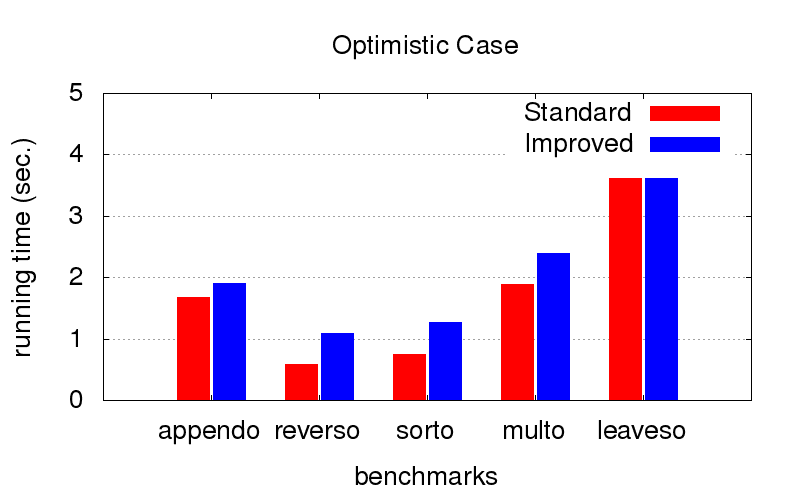
\includegraphics[scale=0.5]{optimistic.png}

\end{frame}

\begin{frame}{Quantitative Evaluation}

  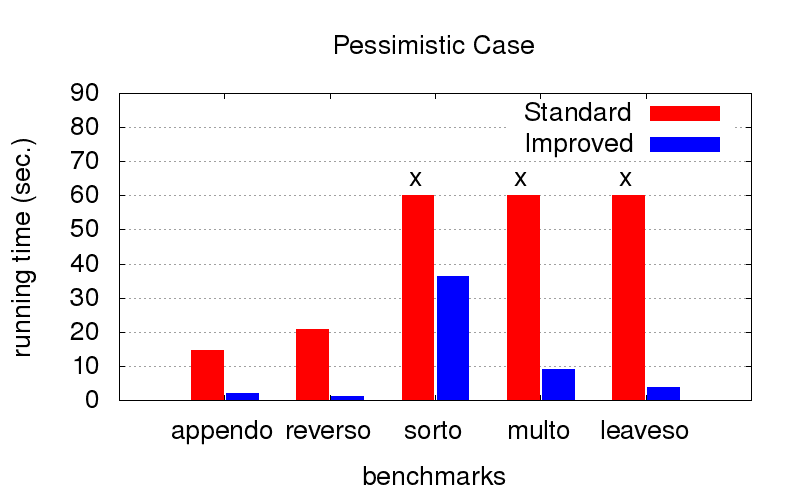
\includegraphics[scale=0.5]{pessimistic.png}

\end{frame}


\begin{frame}{Wrap-up}

\begin{itemize}
 \item A new improved search based on divergence test and conjunct reordering.
 \item Operational semantics for the standard and improved search and proof of convergence preservation.
 \item Performance evaluation: 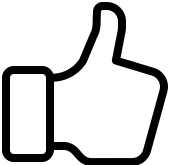
\includegraphics[scale=0.09]{thumbs-up.png} 
\end{itemize}

\end{frame}
\end{document}
